%label:"art:ComparisionToBSide"
%type:"article"
%name:"Comparision to $B$-side"
%caption:""


let $\CritVal(W)\subset C$ be the subset of critical values of $W$. For each $c\in \CritVal(W)$, we have a ``smaller'' Landau-Ginzburg model $Y_c$ by trivially extending the $W^{-1}(B(c, \eps))\to B(c, \eps)$ to a fibration over $\CC$. 
%label:"fig:SmallNeighborhoodFsCategory"
%type:"figure"
%name:"small neighborhood FS category"
%caption:"A small neighborhood in the base of a symplectic LG model can be used to build another LG model."
%parent:"art_ComparisonToBSide"


    \begin{tikzpicture}

        \draw (-3,2.5) rectangle (4,-1.5);
        
        
        \node at (3.5,2) {$\mathbb{C}$};
        
        
        \node at (-1,0) {$\times$};
        \node at (1.5,0.5) {$\times$};
        \node at (-1,1.5) {$\times$};
        \draw[dotted]  (-1,1.5) ellipse (0.5 and 0.5);
        \node at (0,1.5) {$B(c, \epsilon)$};
    \end{tikzpicture}


Define $\FS_c=\FS(Y_v, W)$. 
%label:"def:VanishingPath"
%type:"definition"
%name:"vanishing path"
%caption:""
%parent:"art_ComparisonToBSide"


Let $c \in \CritVal(W)$ be a critical point. A \emph{vanishing path} for $c$ is a path $\gamma: [0, \infty) \to \CC$ such that 
\begin{itemize}
\item $\gamma(0) = c$ 
\item $\gamma$ avoids all other critical values 
\item $\gamma(t) = t$ for $t \gg 0$. 
\end{itemize}


A vanishing path determines an embedding $\FS_c\into \FS(Y, W)$ by extending Lagrangian submanifolds over the vanishing path using symplectic parallel transport. 
%label:"fig:ExtendingByVanishingPath"
%type:"figure"
%name:"extending by vanishing path"
%caption:"A vanishing path determines a method for extending Lagrangians belonging to the Fukaya-Seidel category near a critical value to the Fukaya-Seidel category of $(Y, W)$."
%parent:"art_ComparisonToBSide"


    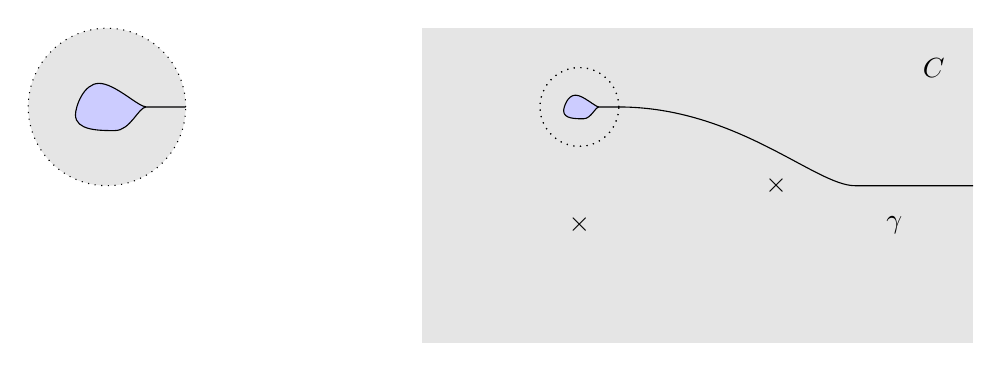
\begin{tikzpicture}

        \fill[gray!20] (-3,2.5) rectangle (4,-1.5);
        
        
        \node at (3.5,2) {$\mathbb{C}$};
        
        
        \node at (-1,0) {$\times$};
        \node at (1.5,0.5) {$\times$};
        \node at (-1,1.5) {$\times$};
        \draw[dotted]  (-1,1.5) ellipse (0.5 and 0.5);
        
        \begin{scope}[]
        \draw[dotted, fill=gray!20] (-7,1.5) ellipse (1 and 1);
        \draw[fill=blue!20] (-6,1.5) .. controls (-6.1,1.5) and (-6.4,1.5) .. (-6.5,1.5) .. controls (-6.6,1.5) and (-6.9,1.8) .. (-7.1,1.8) .. controls (-7.3,1.8) and (-7.4,1.5) .. (-7.4,1.4) .. controls (-7.4,1.2) and (-7.1,1.2) .. (-6.9,1.2) .. controls (-6.7,1.2) and (-6.6,1.5) .. (-6.5,1.5);
        
        \end{scope}
        
        
        \begin{scope}[scale=0.5, shift={(5,1.5)}]
        \draw[dotted] (-7,1.5) ellipse (1 and 1);
        \draw[fill=blue!20] (-6,1.5) .. controls (-6.1,1.5) and (-6.4,1.5) .. (-6.5,1.5) .. controls (-6.6,1.5) and (-6.9,1.8) .. (-7.1,1.8) .. controls (-7.3,1.8) and (-7.4,1.5) .. (-7.4,1.4) .. controls (-7.4,1.2) and (-7.1,1.2) .. (-6.9,1.2) .. controls (-6.7,1.2) and (-6.6,1.5) .. (-6.5,1.5);
        
        \end{scope}
        
        
        \draw (-0.5,1.5) .. controls (1,1.5) and (2,0.5) .. (2.5,0.5) .. controls (3,0.5) and (3.5,0.5) .. (4,0.5);
        \node at (3,0) {$\gamma$};
    \end{tikzpicture}


If we choose ``disjoint'' vanishing paths, we get a semi-orthogonal decomposition.
\[\FS(Y, W) = \langle FS_1, \ldots, FS_n\rangle \]

%label:"exm:MirrorSymmetryForTheProjectivePlane"
%type:"example"
%name:"mirror symmetry for the projective plane"
%caption:""
%parent:"art_ComparisonToBSide"


\label{exm:HMSforP2}
Consider the symplectic Landau-Ginzburg model whose critical points are arranged as follows:
%label:"fig:VanishingPathsForP2"
%type:"figure"
%name:"vanishing paths for P2"
%caption:"A set of vanishing paths for the Lefschetz fibration $W(z_1, z_2) = z_1 + z_2 + (z_1z_2)^{-1}$"
%parent:"exm_MirrorSymmetryForP2"


    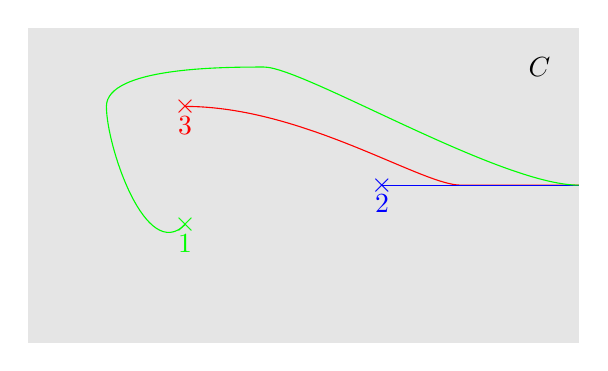
\begin{tikzpicture}

        \fill[gray!20] (-3,2.5) rectangle (4,-1.5);
        
        \node at (3.5,2) {$\mathbb{C}$};
        
        \node[green] at (-1,0) {$\times$};
        \node[blue] at (1.5,0.5) {$\times$};
        \node[red] at (-1,1.5) {$\times$};
        
        \node[below,green] at (-1,0) {$1$};
        \node[below,blue] at (1.5,0.5) {$2$};
        \node[below,red] at (-1,1.5) {$3$};
        \draw[red] (-1,1.5) .. controls (0.5,1.5) and (2,0.5) .. (2.5,0.5) .. controls (3,0.5) and (3.5,0.5) .. (4,0.5);
        \draw[blue] (1.5,0.5) -- (4,0.5);
        \draw[green] (-1,0) .. controls (-1.5,-0.5) and (-2,1) .. (-2,1.5) .. controls (-2,2) and (-0.5,2) .. (0,2) .. controls (0.5,2) and (3,0.5) .. (4,0.5);
    \end{tikzpicture}


 We obtain a semi-orthogonal decomposition $\FS(Y, W) = \langle \FS_1, \FS_2, \FS_3 \rangle$.



